
\chapter{Manifold}

What is manifold? A good example to keep in mind is the surface of a smooth ball. If you look at a small portion of it from very close up, then it looks like a portion of a flat plane. More generally, an $n$-dimensional manifold, is a geometrical object that looks ``locally'' like $n$-dimensional \emph{Euclidean space}.

%In this chapter we give the basic definitions and properties of a smooth manifold and of smooth maps between manifolds. %Initially, the only way we have to verify that a space is a manifold is to exhibit a collection of $C^\infty$-compatible charts covering the space. %In Section \ref{undefined} we describe a set of sufficient conditions under which a quotient topological space becomes a manifold, giving us a second way to construct manifolds.

\section{Topological manifolds}

We first introduce topological manifolds, the most basic type of manifolds. A topological manifold is a space whose each point is surrounded by a region that can be identified with parts of Euclidean space. We may hope that there is a ``nice'' one-to-one map $\varphi$ from the neighborhood into $\mathbf{R}^n$. Then $\varphi$ allows us to use the coordinates in $\mathbf{R}^n$ to label points in the neighborhood: if $p$ belongs to the neighborhood, then one can label it with the coordinates of $\varphi(p)$. This condition is given by the locally Euclidean. The function $\varphi$ is called a coordinate chart of the neighborhood.

\begin{definition}[Topological manifold]
    %Suppose $M$ is a Hausdorff space. If for any $x \in M$, there exists a neighborhood $U$ of $x$ such that $U$ is homeomorphic to an open set in $\mathbf{R}^n$, then $M$ is called an \emph{$n$-dimensional topological manifold} (or \emph{$n$-manifold} for short).
    Suppose $M$ is a topological space. We say that $M$ is an \emph{$n$-dimensional topological manifold} (or a \emph{topological $n$-manifold}) if it has the following properties:
    \begin{enumerate}
        \item $M$ is \emph{Hausdorff}: for every distinct points $x, y \in M$, there exists disjoint open sets $U, V$ such that $x \in U$ and $y \in V$.
        \item $M$ is \emph{second-countable}: $M$ has a countable basis.
        \item $M$ is \emph{locally Euclidean of dimension $n$}: for every $x \in M$, there exists a neighborhood $U$ of $x$ such that $U$ is homeomorphic to an open set in $\mathbf{R}^n$.
    \end{enumerate}
\end{definition}

\begin{remark}
    For the dimension of a topological manifold to be well-defined, we need to know that for $n \neq m$ an open subset of $\mathbf{R}^n$ is not homeomorphic to an open subset of $\mathbf{R}^m$. This fact, called \emph{invariance of dimension}, is indeed true but is not easy to prove directly. Thus, we will not prove the theorem and just leave it here.

\begin{quotation}
    \begin{theorem}[Topological invariance of dimension]\label{lem:topological invariance of dimension}
        A nonempty $n$-dimensional topological manifold cannot be homeomorphic to an $m$-dimensional manifold unless $m = n$.
    \end{theorem}
\end{quotation}
\end{remark}

Now, here is a straightforward but central observation. Suppose that $M$ is a topological manifold of dimension $n$, $U$ and $V$ are two neighborhoods in $M$ that intersect, and suppose that functions $\varphi : U \to \mathbf{R}^n$ and $\psi : V \to \mathbf{R}^n$ are used to give them each a coordinate chart. Then the intersection $U \cap V$ is given two coordinate charts, and this gives us an identification between the open regions $\varphi(U \cap V)$ and $\psi(U \cap V)$ of $\mathbf{R}^n$: given a point $p$ in the first region, the corresponding point in the second is $\psi(\varphi^{-1}(p))$. This composition of maps tells us how the coordinates from one of the charts on the intersecting region relate to those of the other.

\begin{definition}[$C^\infty$-compatible chart]\label{def:compatible chart}
    Let $M$ be a topological $n$-manifold. 
    \begin{itemize}
        \item A \emph{coordinate chart} (or \emph{chart}) on $M$ is a pair $(U, \varphi)$, where $U$ is an open subset of $M$ and $\varphi : U \to \varphi(U)$ is a homeomorphism from $U$ to an open subset $\varphi(U) \subset \mathbf{R}^n$. We say that $(U, \varphi)$ is \emph{centered} at $p \in U$ if $\varphi(p) = 0$.
        \item Two charts $(U, \varphi)$ and $(V, \psi)$ of a topological manifold are \emph{$C^\infty$-compatible} if the two maps
        \begin{align*}
            \varphi \circ \psi^{-1} : \psi(U \cap V) \to \varphi(U \cap V)
            \quad\text{and}\quad
            \psi \circ \varphi^{-1} : \varphi(U \cap V) \to \psi(U \cap V)
        \end{align*}
        are $C^\infty$. This two maps are called the \emph{transition maps} between the charts. 
    \end{itemize}
\end{definition}

\begin{figure}[h]
    \centering
    

% Pattern Info
 
\tikzset{
pattern size/.store in=\mcSize, 
pattern size = 5pt,
pattern thickness/.store in=\mcThickness, 
pattern thickness = 0.3pt,
pattern radius/.store in=\mcRadius, 
pattern radius = 1pt}
\makeatletter
\pgfutil@ifundefined{pgf@pattern@name@_chy5laxe9}{
\pgfdeclarepatternformonly[\mcThickness,\mcSize]{_chy5laxe9}
{\pgfqpoint{0pt}{-\mcThickness}}
{\pgfpoint{\mcSize}{\mcSize}}
{\pgfpoint{\mcSize}{\mcSize}}
{
\pgfsetcolor{\tikz@pattern@color}
\pgfsetlinewidth{\mcThickness}
\pgfpathmoveto{\pgfqpoint{0pt}{\mcSize}}
\pgfpathlineto{\pgfpoint{\mcSize+\mcThickness}{-\mcThickness}}
\pgfusepath{stroke}
}}
\makeatother

% Pattern Info
 
\tikzset{
pattern size/.store in=\mcSize, 
pattern size = 5pt,
pattern thickness/.store in=\mcThickness, 
pattern thickness = 0.3pt,
pattern radius/.store in=\mcRadius, 
pattern radius = 1pt}
\makeatletter
\pgfutil@ifundefined{pgf@pattern@name@_nuxj1x01k}{
\pgfdeclarepatternformonly[\mcThickness,\mcSize]{_nuxj1x01k}
{\pgfqpoint{0pt}{-\mcThickness}}
{\pgfpoint{\mcSize}{\mcSize}}
{\pgfpoint{\mcSize}{\mcSize}}
{
\pgfsetcolor{\tikz@pattern@color}
\pgfsetlinewidth{\mcThickness}
\pgfpathmoveto{\pgfqpoint{0pt}{\mcSize}}
\pgfpathlineto{\pgfpoint{\mcSize+\mcThickness}{-\mcThickness}}
\pgfusepath{stroke}
}}
\makeatother

% Pattern Info
 
\tikzset{
pattern size/.store in=\mcSize, 
pattern size = 5pt,
pattern thickness/.store in=\mcThickness, 
pattern thickness = 0.3pt,
pattern radius/.store in=\mcRadius, 
pattern radius = 1pt}
\makeatletter
\pgfutil@ifundefined{pgf@pattern@name@_s9qe3cxvu}{
\pgfdeclarepatternformonly[\mcThickness,\mcSize]{_s9qe3cxvu}
{\pgfqpoint{0pt}{-\mcThickness}}
{\pgfpoint{\mcSize}{\mcSize}}
{\pgfpoint{\mcSize}{\mcSize}}
{
\pgfsetcolor{\tikz@pattern@color}
\pgfsetlinewidth{\mcThickness}
\pgfpathmoveto{\pgfqpoint{0pt}{\mcSize}}
\pgfpathlineto{\pgfpoint{\mcSize+\mcThickness}{-\mcThickness}}
\pgfusepath{stroke}
}}
\makeatother
\tikzset{every picture/.style={line width=0.75pt}} %set default line width to 0.75pt        

\begin{tikzpicture}[x=0.75pt,y=0.75pt,yscale=-1,xscale=1]
%uncomment if require: \path (0,257); %set diagram left start at 0, and has height of 257

%Shape: Ellipse [id:dp4495052472363552] 
\draw   (245.08,77.59) .. controls (257.66,84.38) and (257.94,107.21) .. (245.69,128.58) .. controls (233.44,149.95) and (213.31,161.77) .. (200.72,154.98) .. controls (188.14,148.18) and (187.87,125.36) .. (200.11,103.99) .. controls (212.36,82.62) and (232.49,70.8) .. (245.08,77.59) -- cycle ;
%Shape: Ellipse [id:dp8595049926507787] 
\draw   (156.32,144.76) .. controls (159.65,131.16) and (182.22,124.72) .. (206.74,130.36) .. controls (231.26,136.01) and (248.45,151.6) .. (245.12,165.19) .. controls (241.8,178.79) and (219.22,185.23) .. (194.7,179.59) .. controls (170.18,173.95) and (153,158.35) .. (156.32,144.76) -- cycle ;
%Shape: Path Data [id:dp016725977566598438] 
\draw  [pattern=_chy5laxe9,pattern size=6pt,pattern thickness=0.75pt,pattern radius=0pt, pattern color={rgb, 255:red, 0; green, 0; blue, 0}] (200.72,154.98) .. controls (192.99,150.8) and (189.91,140.58) .. (191.52,128.35) .. controls (196.4,128.51) and (201.52,129.16) .. (206.74,130.36) .. controls (218.03,132.96) and (227.76,137.66) .. (234.65,143.31) .. controls (223.36,154.88) and (209.99,159.98) .. (200.72,154.98) -- cycle ;
%Shape: Ellipse [id:dp6155554614968932] 
\draw   (357.59,211.13) .. controls (360.92,197.53) and (383.49,191.09) .. (408.01,196.73) .. controls (432.53,202.37) and (449.72,217.97) .. (446.39,231.56) .. controls (443.07,245.16) and (420.5,251.6) .. (395.98,245.96) .. controls (371.46,240.31) and (354.27,224.72) .. (357.59,211.13) -- cycle ;
%Shape: Path Data [id:dp14503763189624563] 
\draw  [pattern=_nuxj1x01k,pattern size=6pt,pattern thickness=0.75pt,pattern radius=0pt, pattern color={rgb, 255:red, 0; green, 0; blue, 0}] (401.99,221.34) .. controls (394.26,217.17) and (391.18,206.94) .. (392.79,194.72) .. controls (397.67,194.87) and (402.8,195.53) .. (408.01,196.73) .. controls (419.3,199.33) and (429.03,204.03) .. (435.92,209.68) .. controls (424.63,221.25) and (411.26,226.35) .. (401.99,221.34) -- cycle ;
%Shape: Ellipse [id:dp7131547008704517] 
\draw   (429.18,9.61) .. controls (441.76,16.4) and (442.04,39.23) .. (429.79,60.6) .. controls (417.54,81.97) and (397.41,93.79) .. (384.82,87) .. controls (372.24,80.21) and (371.97,57.38) .. (384.21,36.01) .. controls (396.46,14.64) and (416.59,2.82) .. (429.18,9.61) -- cycle ;
%Shape: Path Data [id:dp7287392242053876] 
\draw  [pattern=_s9qe3cxvu,pattern size=6pt,pattern thickness=0.75pt,pattern radius=0pt, pattern color={rgb, 255:red, 0; green, 0; blue, 0}] (384.82,87) .. controls (377.09,82.82) and (374.01,72.6) .. (375.62,60.37) .. controls (380.5,60.53) and (385.62,61.18) .. (390.84,62.38) .. controls (402.13,64.98) and (411.86,69.68) .. (418.75,75.33) .. controls (407.46,86.9) and (394.09,92) .. (384.82,87) -- cycle ;
%Curve Lines [id:da6430898730655943] 
\draw    (250,74) .. controls (269.8,41.33) and (329.78,24.34) .. (371.73,42.44) ;
\draw [shift={(373,43)}, rotate = 204.34] [color={rgb, 255:red, 0; green, 0; blue, 0 }  ][line width=0.75]    (10.93,-3.29) .. controls (6.95,-1.4) and (3.31,-0.3) .. (0,0) .. controls (3.31,0.3) and (6.95,1.4) .. (10.93,3.29)   ;
%Curve Lines [id:da04465891427013591] 
\draw    (240,179) .. controls (249.9,222.56) and (294.1,242.6) .. (348.35,223.59) ;
\draw [shift={(350,223)}, rotate = 160.02] [color={rgb, 255:red, 0; green, 0; blue, 0 }  ][line width=0.75]    (10.93,-3.29) .. controls (6.95,-1.4) and (3.31,-0.3) .. (0,0) .. controls (3.31,0.3) and (6.95,1.4) .. (10.93,3.29)   ;
%Curve Lines [id:da6875480561506901] 
\draw    (377,98) .. controls (357.4,125.44) and (359.89,155.76) .. (369.41,182.38) ;
\draw [shift={(370,184)}, rotate = 249.68] [color={rgb, 255:red, 0; green, 0; blue, 0 }  ][line width=0.75]    (10.93,-3.29) .. controls (6.95,-1.4) and (3.31,-0.3) .. (0,0) .. controls (3.31,0.3) and (6.95,1.4) .. (10.93,3.29)   ;
%Curve Lines [id:da947482143477028] 
\draw    (399,185) .. controls (411.81,166.29) and (417.82,133.02) .. (404.62,99.53) ;
\draw [shift={(404,98)}, rotate = 67.62] [color={rgb, 255:red, 0; green, 0; blue, 0 }  ][line width=0.75]    (10.93,-3.29) .. controls (6.95,-1.4) and (3.31,-0.3) .. (0,0) .. controls (3.31,0.3) and (6.95,1.4) .. (10.93,3.29)   ;
%Curve Lines [id:da12726184143888863] 
\draw    (89,114) .. controls (116,131) and (148,104) .. (149,81) ;
%Shape: Polygon Curved [id:ds0665293937289353] 
\draw   (99,74) .. controls (169,66) and (215,30) .. (256,67) .. controls (297,104) and (290,153) .. (257,181) .. controls (224,209) and (146,205) .. (97,176) .. controls (48,147) and (29,82) .. (99,74) -- cycle ;
%Curve Lines [id:da8322855942345793] 
\draw    (100,118) .. controls (93,96) and (131,74) .. (146,93) ;

% Text Node
\draw (228,80.4) node [anchor=north west][inner sep=0.75pt]    {$\mathnormal{U}$};
% Text Node
\draw (175,98.4) node [anchor=north west][inner sep=0.75pt]    {$M$};
% Text Node
\draw (214,160.4) node [anchor=north west][inner sep=0.75pt]    {$V$};
% Text Node
\draw (288,17.4) node [anchor=north west][inner sep=0.75pt]    {$\varphi $};
% Text Node
\draw (274,231.4) node [anchor=north west][inner sep=0.75pt]    {$\psi $};
% Text Node
\draw (382,45.4) node [anchor=north west][inner sep=0.75pt]  [font=\scriptsize]  {$\varphi ( U\cap V)$};
% Text Node
\draw (389,227.4) node [anchor=north west][inner sep=0.75pt]  [font=\scriptsize]  {$\psi ( U\cap V)$};
% Text Node
\draw (417,135.4) node [anchor=north west][inner sep=0.75pt]    {$\varphi \circ \psi ^{-1}$};
% Text Node
\draw (308,134.4) node [anchor=north west][inner sep=0.75pt]    {$\psi \circ \varphi ^{-1}$};


\end{tikzpicture}

    \caption{Transition maps (see Definition \ref{def:compatible chart})}
\end{figure}

Given a topological $n$-manifold $M$, and a chart $(U, \varphi)$ containing $p \in M$. Since $\varphi$ is a homeomorphism, for any $p \in U$, we can define the coordinate of $p$ to be the coordinate of $\varphi(p) \in \mathbf{R}^n$. Specifically, let $y_1, \cdots, y_n$ be the coordinates on $\mathbf{R}^n$, we let $x_i = y_i \circ \varphi$ be the $i$th component of $\varphi$ and write $\varphi(p) = (x_1(p), \cdots, x_n(p))$. Thus, for $p \in U$, $(x_1(p), \cdots, x_n(p))$ is a point in $\mathbf{R}^n$. The functions $x_1, \cdots, x_n$ are called \emph{local coordinates} on $U$.

Here is some simple examples of topological manifolds.

\begin{example}[Euclidean sapce]
    The Euclidean space $\mathbf{R}^n$ is covered by a single chart $(\mathbf{R}^n, \id_{\mathbf{R}^n})$, where $\id_{\mathbf{R}^n}$ is the identity map of $\mathbf{R}^n$. Every open subset $U$ of $\mathbf{R}^n$ is also a topological manifold with chart $(U, \id_U)$.
\end{example}

\begin{example}[Graphs of continuous functions]
    Let $U \subset \mathbf{R}^n$ be an open subset, and let $f : U \to \mathbf{R}^k$ be a continuous function. The graph of $f$ is the subset of $\mathbf{R}^n \times \mathbf{R}^k$ defined by
    \begin{align*}
        \Gamma(f) := \{(x, y) \in \mathbf{R}^n \times \mathbf{R}^k : x \in U, y = f(x)\},
    \end{align*}
    with the subspace topology. Let $\pi_1 : \mathbf{R}^n \times \mathbf{R}^k \to \mathbf{R}^n$ denote the projection onto the first component.
\end{example}

\begin{example}[Spheres]
    For each $n \geq 0$, the unit $n$-sphere $\mathbf{S}^n$ is Hausdorff and second-countable because it is a topological subspace of $\mathbf{R}^{n + 1}$. To show that it is locally Euclidean, for each $1 \leq i \leq n + 1$, let $U_i^+$ denote the subset of $\mathbf{R}^{n + 1}$ where the $i$th coordinate is positive:
    \begin{align*}
        U_i^+ := \{(x_1, \cdots, x_{n + 1}) \in \mathbf{R}^{n + 1} : x_i > 0\}.
    \end{align*}
    Similarly, $U_i^-$ is the set where $x_i < 0$.

    Let $\mathbf{B}^n$ be the set of open unit balls in $\mathbf{R}^n$, and let $f : \mathbf{B}^n \to \mathbf{R}$ be the continuous function
    \begin{align*}
        f(u) = \sqrt{1 - \|u\|^2}.
    \end{align*}
\end{example}

\begin{example}[Projective spaces]
    
\end{example}


\section{Smooth structures}

There are no constraints on the coordinate chart maps on a topological manifold except that they should be continuous. However, some continuous functions are quite unpleasant, so one typically introduces extra constraints that the coordinate chart maps are infinitely differentiable. If a manifold has a collection of charts for which all the coordinate chart maps are $C^\infty$, then it is said to have a \emph{smooth differentiable structure}, and it is called a \emph{smooth manifold}. Smooth manifolds are especially interesting because they are the natural arena for calculus. Roughly speaking, they are the most general context in which the notion of differentiation to any order makes intrinsic sense.

\begin{comment}
\begin{definition}[Atlas]
    A \emph{$C^\infty$-atlas} (or an \emph{atlas}) on a locally Euclidean space $M$ is a collection $\mathfrak{A} = \{(U_\alpha, \varphi_\alpha)\}$ of pairwise $C^\infty$-compatible charts that cover $M$, i.e., such that $M = \bigcup_{\alpha}U_\alpha$.
\end{definition}

\begin{lemma}
    Let $\{(U_\alpha, \varphi_\alpha)\}$ be an atlas on a locally Euclidean space. If two charts $(V, \varrho)$ and $(W, \psi)$ are both compatible with the atlas $\{(U_\alpha, \varphi_\alpha)\}$, then they are compatible with each other.
\end{lemma}

\begin{proof}
    Let $p \in V \cap W$. We need to show that $\psi \circ \varrho^{-1}$ is $C^\infty$ at $\varrho(p)$. Since $\{(U_\alpha, \varphi_\alpha)\}$ is an atlas for $M$, $p \in U_\alpha$ for some $\alpha$. Then $p \in U_\alpha \cap V \cap W$.
\end{proof}
\end{comment}

\begin{definition}[$C^\infty$-differentiable structure]
    Let $M$ be a topological $n$-manifold. If given a collection of charts $\mathfrak{A} = \{(U_\alpha, \varphi_\alpha)\}$ on $M$ satisfies the following conditions, then we call $\mathfrak{A}$ a \emph{$C^\infty$-differentiable structure} on $M$:
    \begin{enumerate}
        \item $\mathfrak{A}$ covers $M$, i.e., $M = \bigcup_\alpha U_\alpha$.
        \item Any two charts in $\mathfrak{A}$ are $C^\infty$-compatible.
        \item $\mathfrak{A}$ is \emph{maximal}, i.e., if a chart $(V, \psi)$ is $C^\infty$-compatible with all charts in $\mathfrak{A}$, then $(V, \psi) \in \mathfrak{A}$.
    \end{enumerate}

    The collection of charts $\mathfrak{A}$ is called a \emph{$C^\infty$-atlas} for $M$ if it satisfying condition (i) and (ii). Therefore, A \emph{$C^\infty$-differentiable structure} on $M$ is a maximal atlas on $M$.
\end{definition}

\begin{definition}[Smooth manifold]
    Let $M$ be a topological $n$-manifold. If a $C^\infty$-differentiable structure is given on $M$, then $M$ is called a \emph{$C^\infty$-manifold of dimension $n$} (or a \emph{smooth $n$-manifold}).
\end{definition}

In practice, to check that a topological manifold $M$ is a smooth manifold, it is not necessary to exhibit a maximal atlas. The existence of any atlas on $M$ will do, because of the following proposition.

\begin{proposition}\label{lem:condition of smooth manifold}
    Let $M$ be a topological manifold. Every atlas $\mathfrak{A} = \{(U_\alpha, \varphi_\alpha)\}$ for $M$ is contained in a unique maximal atlas.
\end{proposition}

\begin{proof}
    Let $\mathfrak{A}$ be a $C^\infty$-atlas for $M$, and let $\mathfrak{M}$ be the set of all charts that are $C^\infty$-compatible with every chart in $\mathfrak{A}$. We first show that $\mathfrak{M}$ is a $C^\infty$-atlas, we need to show that any two charts in $\mathfrak{M}$ are $C^\infty$-compatible with each other. Let $(U, \varphi), (V, \psi) \in \mathfrak{M}$, we need to show that $\psi \circ \varphi^{-1} : \varphi(U \cap V) \to \psi(U \cap V)$ is $C^\infty$.

    \begin{figure}[h]
        \centering
        
% Pattern Info
 
\tikzset{
pattern size/.store in=\mcSize, 
pattern size = 5pt,
pattern thickness/.store in=\mcThickness, 
pattern thickness = 0.3pt,
pattern radius/.store in=\mcRadius, 
pattern radius = 1pt}
\makeatletter
\pgfutil@ifundefined{pgf@pattern@name@_2ff90oiep}{
\pgfdeclarepatternformonly[\mcThickness,\mcSize]{_2ff90oiep}
{\pgfqpoint{0pt}{-\mcThickness}}
{\pgfpoint{\mcSize}{\mcSize}}
{\pgfpoint{\mcSize}{\mcSize}}
{
\pgfsetcolor{\tikz@pattern@color}
\pgfsetlinewidth{\mcThickness}
\pgfpathmoveto{\pgfqpoint{0pt}{\mcSize}}
\pgfpathlineto{\pgfpoint{\mcSize+\mcThickness}{-\mcThickness}}
\pgfusepath{stroke}
}}
\makeatother

% Pattern Info
 
\tikzset{
pattern size/.store in=\mcSize, 
pattern size = 5pt,
pattern thickness/.store in=\mcThickness, 
pattern thickness = 0.3pt,
pattern radius/.store in=\mcRadius, 
pattern radius = 1pt}
\makeatletter
\pgfutil@ifundefined{pgf@pattern@name@_gsk3k7a7l}{
\pgfdeclarepatternformonly[\mcThickness,\mcSize]{_gsk3k7a7l}
{\pgfqpoint{0pt}{-\mcThickness}}
{\pgfpoint{\mcSize}{\mcSize}}
{\pgfpoint{\mcSize}{\mcSize}}
{
\pgfsetcolor{\tikz@pattern@color}
\pgfsetlinewidth{\mcThickness}
\pgfpathmoveto{\pgfqpoint{0pt}{\mcSize}}
\pgfpathlineto{\pgfpoint{\mcSize+\mcThickness}{-\mcThickness}}
\pgfusepath{stroke}
}}
\makeatother

% Pattern Info
 
\tikzset{
pattern size/.store in=\mcSize, 
pattern size = 5pt,
pattern thickness/.store in=\mcThickness, 
pattern thickness = 0.3pt,
pattern radius/.store in=\mcRadius, 
pattern radius = 1pt}
\makeatletter
\pgfutil@ifundefined{pgf@pattern@name@_08pqtiufy}{
\pgfdeclarepatternformonly[\mcThickness,\mcSize]{_08pqtiufy}
{\pgfqpoint{0pt}{-\mcThickness}}
{\pgfpoint{\mcSize}{\mcSize}}
{\pgfpoint{\mcSize}{\mcSize}}
{
\pgfsetcolor{\tikz@pattern@color}
\pgfsetlinewidth{\mcThickness}
\pgfpathmoveto{\pgfqpoint{0pt}{\mcSize}}
\pgfpathlineto{\pgfpoint{\mcSize+\mcThickness}{-\mcThickness}}
\pgfusepath{stroke}
}}
\makeatother

% Pattern Info
 
\tikzset{
pattern size/.store in=\mcSize, 
pattern size = 5pt,
pattern thickness/.store in=\mcThickness, 
pattern thickness = 0.3pt,
pattern radius/.store in=\mcRadius, 
pattern radius = 1pt}
\makeatletter
\pgfutil@ifundefined{pgf@pattern@name@_gzbpehfbb}{
\pgfdeclarepatternformonly[\mcThickness,\mcSize]{_gzbpehfbb}
{\pgfqpoint{0pt}{-\mcThickness}}
{\pgfpoint{\mcSize}{\mcSize}}
{\pgfpoint{\mcSize}{\mcSize}}
{
\pgfsetcolor{\tikz@pattern@color}
\pgfsetlinewidth{\mcThickness}
\pgfpathmoveto{\pgfqpoint{0pt}{\mcSize}}
\pgfpathlineto{\pgfpoint{\mcSize+\mcThickness}{-\mcThickness}}
\pgfusepath{stroke}
}}
\makeatother
\tikzset{every picture/.style={line width=0.75pt}} %set default line width to 0.75pt        

\begin{tikzpicture}[x=0.75pt,y=0.75pt,yscale=-1,xscale=1]
%uncomment if require: \path (0,389); %set diagram left start at 0, and has height of 389

%Shape: Ellipse [id:dp9751170753695928] 
\draw   (290.22,64.83) .. controls (297.99,56.98) and (315.43,61.63) .. (329.17,75.23) .. controls (342.91,88.83) and (347.75,106.21) .. (339.98,114.06) .. controls (332.21,121.92) and (314.77,117.26) .. (301.03,103.66) .. controls (287.29,90.07) and (282.45,72.68) .. (290.22,64.83) -- cycle ;
%Shape: Ellipse [id:dp8236698722694553] 
\draw   (374.87,68.23) .. controls (381.93,76.72) and (375.61,93.62) .. (360.75,105.98) .. controls (345.89,118.34) and (328.11,121.48) .. (321.05,112.99) .. controls (313.99,104.49) and (320.31,87.59) .. (335.17,75.23) .. controls (350.03,62.87) and (367.81,59.73) .. (374.87,68.23) -- cycle ;
%Shape: Ellipse [id:dp00022545106876314946] 
\draw   (331.49,88) .. controls (342.53,88.16) and (351.27,103.95) .. (351,123.28) .. controls (350.73,142.61) and (341.56,158.15) .. (330.51,158) .. controls (319.47,157.84) and (310.73,142.05) .. (311,122.72) .. controls (311.27,103.39) and (320.44,87.85) .. (331.49,88) -- cycle ;
%Curve Lines [id:da024755229005684276] 
\draw    (214,86) .. controls (241,103) and (273,76) .. (274,53) ;
%Shape: Polygon Curved [id:ds3029869656856743] 
\draw   (224,46) .. controls (294,38) and (340,2) .. (381,39) .. controls (422,76) and (415,125) .. (382,153) .. controls (349,181) and (271,177) .. (222,148) .. controls (173,119) and (154,54) .. (224,46) -- cycle ;
%Curve Lines [id:da1900501825763503] 
\draw    (225,90) .. controls (218,68) and (256,46) .. (271,65) ;
%Shape: Path Data [id:dp40215485030273945] 
\draw  [pattern=_2ff90oiep,pattern size=6pt,pattern thickness=0.75pt,pattern radius=0pt, pattern color={rgb, 255:red, 0; green, 0; blue, 0}] (339.98,114.06) .. controls (337.91,116.15) and (335.16,117.36) .. (331.98,117.74) .. controls (327.4,117.55) and (323.55,116) .. (321.05,112.99) .. controls (317.08,108.22) and (317.34,100.8) .. (320.95,93.03) .. controls (324.04,89.79) and (327.65,87.95) .. (331.49,88) .. controls (335.03,88.05) and (338.33,89.71) .. (341.17,92.57) .. controls (344.76,101.25) and (344.63,109.36) .. (339.98,114.06) -- cycle ;
%Shape: Ellipse [id:dp9480763091871542] 
\draw   (330.49,253) .. controls (341.53,253.16) and (350.27,268.95) .. (350,288.28) .. controls (349.73,307.61) and (340.56,323.15) .. (329.51,323) .. controls (318.47,322.84) and (309.73,307.05) .. (310,287.72) .. controls (310.27,268.39) and (319.44,252.85) .. (330.49,253) -- cycle ;
%Shape: Path Data [id:dp16425278831533818] 
\draw  [pattern=_gsk3k7a7l,pattern size=6pt,pattern thickness=0.75pt,pattern radius=0pt, pattern color={rgb, 255:red, 0; green, 0; blue, 0}] (338.98,279.06) .. controls (336.91,281.15) and (334.16,282.36) .. (330.98,282.74) .. controls (326.4,282.55) and (322.55,281) .. (320.05,277.99) .. controls (316.08,273.22) and (316.34,265.8) .. (319.95,258.03) .. controls (323.04,254.79) and (326.65,252.95) .. (330.49,253) .. controls (334.03,253.05) and (337.33,254.71) .. (340.17,257.57) .. controls (343.76,266.25) and (343.63,274.36) .. (338.98,279.06) -- cycle ;
%Shape: Ellipse [id:dp3134718727172334] 
\draw   (495.87,267.23) .. controls (502.93,275.72) and (496.61,292.62) .. (481.75,304.98) .. controls (466.89,317.34) and (449.11,320.48) .. (442.05,311.99) .. controls (434.99,303.49) and (441.31,286.59) .. (456.17,274.23) .. controls (471.03,261.87) and (488.81,258.73) .. (495.87,267.23) -- cycle ;
%Shape: Path Data [id:dp6347059658428231] 
\draw  [pattern=_08pqtiufy,pattern size=6pt,pattern thickness=0.75pt,pattern radius=0pt, pattern color={rgb, 255:red, 0; green, 0; blue, 0}] (460.98,313.06) .. controls (458.91,315.15) and (456.16,316.36) .. (452.98,316.74) .. controls (448.4,316.55) and (444.55,315) .. (442.05,311.99) .. controls (438.08,307.22) and (438.34,299.8) .. (441.95,292.03) .. controls (445.04,288.79) and (448.65,286.95) .. (452.49,287) .. controls (456.03,287.05) and (459.33,288.71) .. (462.17,291.57) .. controls (465.76,300.25) and (465.63,308.36) .. (460.98,313.06) -- cycle ;
%Shape: Path Data [id:dp519960467674657] 
\draw  [dash pattern={on 0.84pt off 2.51pt}] (190.98,316.06) .. controls (188.91,318.15) and (186.16,319.36) .. (182.98,319.74) .. controls (178.4,319.55) and (174.55,318) .. (172.05,314.99) .. controls (165.53,307.14) and (170.42,292.12) .. (182.92,280.13) .. controls (194.52,293.21) and (198.21,308.76) .. (190.98,316.06) -- cycle ;
%Shape: Path Data [id:dp11425313260516057] 
\draw  [pattern=_gzbpehfbb,pattern size=6pt,pattern thickness=0.75pt,pattern radius=0pt, pattern color={rgb, 255:red, 0; green, 0; blue, 0}] (190.98,316.06) .. controls (188.91,318.15) and (186.16,319.36) .. (182.98,319.74) .. controls (178.4,319.55) and (174.55,318) .. (172.05,314.99) .. controls (168.08,310.22) and (168.34,302.8) .. (171.95,295.03) .. controls (175.04,291.79) and (178.65,289.95) .. (182.49,290) .. controls (186.03,290.05) and (189.33,291.71) .. (192.17,294.57) .. controls (195.76,303.25) and (195.63,311.36) .. (190.98,316.06) -- cycle ;
%Shape: Path Data [id:dp8319909502027762] 
\draw  [dash pattern={on 0.84pt off 2.51pt}] (460.98,313.06) .. controls (458.91,315.15) and (456.16,316.36) .. (452.98,316.74) .. controls (448.4,316.55) and (444.55,315) .. (442.05,311.99) .. controls (435.53,304.14) and (440.42,289.12) .. (452.92,277.13) .. controls (464.52,290.21) and (468.21,305.76) .. (460.98,313.06) -- cycle ;
%Shape: Path Data [id:dp9553001643979384] 
\draw  [dash pattern={on 0.84pt off 2.51pt}] (442.05,311.99) .. controls (438.08,307.22) and (438.34,299.8) .. (441.95,292.03) .. controls (445.04,288.79) and (448.65,286.95) .. (452.49,287) .. controls (461.49,287.13) and (468.95,297.64) .. (471.26,311.98) .. controls (459.32,318.17) and (447.5,318.54) .. (442.05,311.99) -- cycle ;
%Shape: Ellipse [id:dp6645431577061451] 
\draw   (141.22,266.83) .. controls (148.99,258.98) and (166.43,263.63) .. (180.17,277.23) .. controls (193.91,290.83) and (198.75,308.21) .. (190.98,316.06) .. controls (183.21,323.92) and (165.77,319.26) .. (152.03,305.66) .. controls (138.29,292.07) and (133.45,274.68) .. (141.22,266.83) -- cycle ;
%Shape: Path Data [id:dp049768931828376495] 
\draw  [dash pattern={on 0.84pt off 2.51pt}] (190.98,316.07) .. controls (185.19,321.91) and (174.05,320.82) .. (163.06,314.27) .. controls (165.8,300.09) and (173.53,289.88) .. (182.49,290) .. controls (186.03,290.05) and (189.33,291.71) .. (192.17,294.57) .. controls (195.76,303.25) and (195.63,311.36) .. (190.98,316.07) -- cycle ;
%Shape: Path Data [id:dp37637155489000795] 
\draw  [dash pattern={on 0.84pt off 2.51pt}] (338.98,279.06) .. controls (333.19,284.91) and (322.05,283.82) .. (311.06,277.27) .. controls (313.8,263.09) and (321.53,252.88) .. (330.49,253) .. controls (334.03,253.05) and (337.33,254.71) .. (340.17,257.57) .. controls (343.76,266.25) and (343.63,274.36) .. (338.98,279.06) -- cycle ;
%Shape: Path Data [id:dp44097825368255594] 
\draw  [dash pattern={on 0.84pt off 2.51pt}] (320.05,277.99) .. controls (316.08,273.22) and (316.34,265.8) .. (319.95,258.03) .. controls (323.04,254.79) and (326.65,252.95) .. (330.49,253) .. controls (339.49,253.13) and (346.95,263.64) .. (349.26,277.98) .. controls (337.32,284.17) and (325.5,284.54) .. (320.05,277.99) -- cycle ;
%Shape: Circle [id:dp7795223965994169] 
\draw  [fill={rgb, 255:red, 0; green, 0; blue, 0 }  ,fill opacity=1 ] (328,98.5) .. controls (328,97.12) and (329.12,96) .. (330.5,96) .. controls (331.88,96) and (333,97.12) .. (333,98.5) .. controls (333,99.88) and (331.88,101) .. (330.5,101) .. controls (329.12,101) and (328,99.88) .. (328,98.5) -- cycle ;

%Curve Lines [id:da7823801932441379] 
\draw    (282,101) .. controls (210.72,122.78) and (170.8,197.49) .. (176.8,258.17) ;
\draw [shift={(177,260)}, rotate = 263.45] [color={rgb, 255:red, 0; green, 0; blue, 0 }  ][line width=0.75]    (10.93,-3.29) .. controls (6.95,-1.4) and (3.31,-0.3) .. (0,0) .. controls (3.31,0.3) and (6.95,1.4) .. (10.93,3.29)   ;
%Curve Lines [id:da3298590078397039] 
\draw    (375,103) .. controls (430.44,135.67) and (455.5,194.8) .. (456.96,256.14) ;
\draw [shift={(457,258)}, rotate = 269.08] [color={rgb, 255:red, 0; green, 0; blue, 0 }  ][line width=0.75]    (10.93,-3.29) .. controls (6.95,-1.4) and (3.31,-0.3) .. (0,0) .. controls (3.31,0.3) and (6.95,1.4) .. (10.93,3.29)   ;
%Curve Lines [id:da3854265371499428] 
\draw    (329,163) .. controls (330.96,186.52) and (329.08,215.8) .. (329.94,243.32) ;
\draw [shift={(330,245)}, rotate = 267.95] [color={rgb, 255:red, 0; green, 0; blue, 0 }  ][line width=0.75]    (10.93,-3.29) .. controls (6.95,-1.4) and (3.31,-0.3) .. (0,0) .. controls (3.31,0.3) and (6.95,1.4) .. (10.93,3.29)   ;
%Curve Lines [id:da7466428971346617] 
\draw    (191,269) .. controls (218.58,245.36) and (261.68,247.92) .. (298.33,266.16) ;
\draw [shift={(300,267)}, rotate = 207.18] [color={rgb, 255:red, 0; green, 0; blue, 0 }  ][line width=0.75]    (10.93,-3.29) .. controls (6.95,-1.4) and (3.31,-0.3) .. (0,0) .. controls (3.31,0.3) and (6.95,1.4) .. (10.93,3.29)   ;
%Curve Lines [id:da5387107494263412] 
\draw    (356,270) .. controls (381.61,249.32) and (415.95,249.97) .. (442.78,269.11) ;
\draw [shift={(444,270)}, rotate = 216.53] [color={rgb, 255:red, 0; green, 0; blue, 0 }  ][line width=0.75]    (10.93,-3.29) .. controls (6.95,-1.4) and (3.31,-0.3) .. (0,0) .. controls (3.31,0.3) and (6.95,1.4) .. (10.93,3.29)   ;
%Shape: Circle [id:dp9143510744897032] 
\draw  [fill={rgb, 255:red, 0; green, 0; blue, 0 }  ,fill opacity=1 ] (179,302.5) .. controls (179,301.12) and (180.12,300) .. (181.5,300) .. controls (182.88,300) and (184,301.12) .. (184,302.5) .. controls (184,303.88) and (182.88,305) .. (181.5,305) .. controls (180.12,305) and (179,303.88) .. (179,302.5) -- cycle ;
%Straight Lines [id:da19315524771135406] 
\draw    (182,326) -- (181.55,307) ;
\draw [shift={(181.5,305)}, rotate = 88.64] [color={rgb, 255:red, 0; green, 0; blue, 0 }  ][line width=0.75]    (10.93,-3.29) .. controls (6.95,-1.4) and (3.31,-0.3) .. (0,0) .. controls (3.31,0.3) and (6.95,1.4) .. (10.93,3.29)   ;
%Curve Lines [id:da3942705805991875] 
\draw    (203,318) .. controls (246.56,347.7) and (380.29,354.86) .. (430.5,322.01) ;
\draw [shift={(432,321)}, rotate = 145.24] [color={rgb, 255:red, 0; green, 0; blue, 0 }  ][line width=0.75]    (10.93,-3.29) .. controls (6.95,-1.4) and (3.31,-0.3) .. (0,0) .. controls (3.31,0.3) and (6.95,1.4) .. (10.93,3.29)   ;

% Text Node
\draw (332,40.4) node [anchor=north west][inner sep=0.75pt]    {$\mathnormal{M}$};
% Text Node
\draw (292.22,68.23) node [anchor=north west][inner sep=0.75pt]    {$U$};
% Text Node
\draw (354,70.4) node [anchor=north west][inner sep=0.75pt]    {$V$};
% Text Node
\draw (319,134.4) node [anchor=north west][inner sep=0.75pt]    {$W$};
% Text Node
\draw (325,100.4) node [anchor=north west][inner sep=0.75pt]  [font=\small]  {$p$};
% Text Node
\draw (176,159.4) node [anchor=north west][inner sep=0.75pt]    {$\varphi $};
% Text Node
\draw (444,158.4) node [anchor=north west][inner sep=0.75pt]    {$\psi $};
% Text Node
\draw (312,194.4) node [anchor=north west][inner sep=0.75pt]    {$\varrho $};
% Text Node
\draw (226,226.4) node [anchor=north west][inner sep=0.75pt]    {$\varrho \circ \varphi ^{-1}$};
% Text Node
\draw (378,230.4) node [anchor=north west][inner sep=0.75pt]    {$\psi \circ \varrho ^{-1}$};
% Text Node
\draw (170,327.4) node [anchor=north west][inner sep=0.75pt]  [font=\footnotesize]  {$\varphi ( p)$};
% Text Node
\draw (260,350.4) node [anchor=north west][inner sep=0.75pt]    {$\left( \psi \circ \varrho ^{-1}\right) \circ \left( \varrho \circ \varphi ^{-1}\right)$};


\end{tikzpicture}

        \caption{Proof of Proposition \ref{lem:condition of smooth manifold}}
    \end{figure}

    Let $\varphi(p) \in \varphi(U \cap V)$ be arbitrary. Since $\bigcup\mathfrak{A} = M$, there is a chart $(W, \varrho) \in \mathfrak{A}$ such that $p \in W$. Since every chart in $\mathfrak{M}$ is $C^\infty$-compatible with $(W, \varrho)$, both of the maps $\varrho \circ \varphi^{-1}$ and $\psi \circ \varrho^{-1}$ are $C^\infty$. Since $p \in U \cap V \cap W$, we have $\psi \circ \varphi^{-1} = (\psi \circ \varrho^{-1}) \circ (\varrho \circ \varphi^{-1})$ is $C^\infty$ on a neighborhood of $\varphi(p)$. Since $\varphi(p)$ is arbitrary, $\psi \circ \varphi^{-1}$ is $C^\infty$ in a neighborhood of each point of $\varphi(U \cap V)$. This is similar to show that $\varphi \circ \psi^{-1}$ is $C^\infty$ on $\psi(U \cap V)$. Thus $\mathfrak{M}$ is a $C^\infty$-atlas.

    The existence of the maximal atlas $\mathfrak{M}$ is given the definition of $\mathfrak{M}$ and $\mathfrak{A} \subset \mathfrak{M}$. To check that $\mathfrak{M}$ is unique, suppose that $\mathfrak{N}$ be any other maximal atlas that containing $\mathfrak{A}$. Then each charts in $\mathfrak{N}$ is $C^\infty$-compatible with each charts in $\mathfrak{A}$, hence $\mathfrak{N} \subset \mathfrak{M}$. Other hand, since $\mathfrak{N}$ is maximal, we have $\mathfrak{N} \supset \mathfrak{M}$. Thus, $\mathfrak{N} = \mathfrak{M}$.
\end{proof}

Since a $C^\infty$-atlas for $M$ covers $M$, Proposition \ref{lem:condition of smooth manifold} shows that it suffices to verify $M$ to be a smooth manifold if it satisfying
\begin{enumerate}
    \item $M$ is Hausdorff and second countable.
    \item $M$ has a $C^\infty$-atlas (not necessarily to be maximal).
\end{enumerate}

\begin{notation}
    When we say a chart on a manifold, we mean a chart in the differentiable structure of manifold.
\end{notation}

\subsection{Examples of smooth manifolds}

\begin{example}[Euclidean spaces]
    The Euclidean space $\mathbf{R}^n$ is a smooth $n$-manifold with the smooth structure determined by the atlas consisting of the single chart $(\mathbf{R}^n, \id_{\mathbf{R}^n})$. We call this the \emph{standard smooth structure on $\mathbf{R}^n$} and the resulting coordinate map \emph{standard coordinates}.
\end{example}



\section{Smooth maps}

\subsection{Smooth functions on manifold}
On a smooth manifold, the concept of a smooth function is well-defined.
\begin{definition}[Smooth function]
    Let $M$ be a smooth manifold of dimension $n$, and let $f : M \to \mathbf{R}^d$ be a function. If $p \in M$, We say that $f$ is $C^\infty$ or \emph{smooth at $p$} if there exists a chart $(U, \varphi)$ containing $p$ such that $f \circ \varphi^{-1}$ is $C^\infty$ at $\varphi(p)$ on the open set $\varphi(U) \subset \mathbf{R}^n$. We say that $f$ is \emph{smooth} if it is smooth at every point of $M$. We denote the set of all smooth functions on $M$ by $C^\infty(M)$.
\end{definition}

\begin{figure}[h]
    \centering
    

\tikzset{every picture/.style={line width=0.75pt}} %set default line width to 0.75pt        

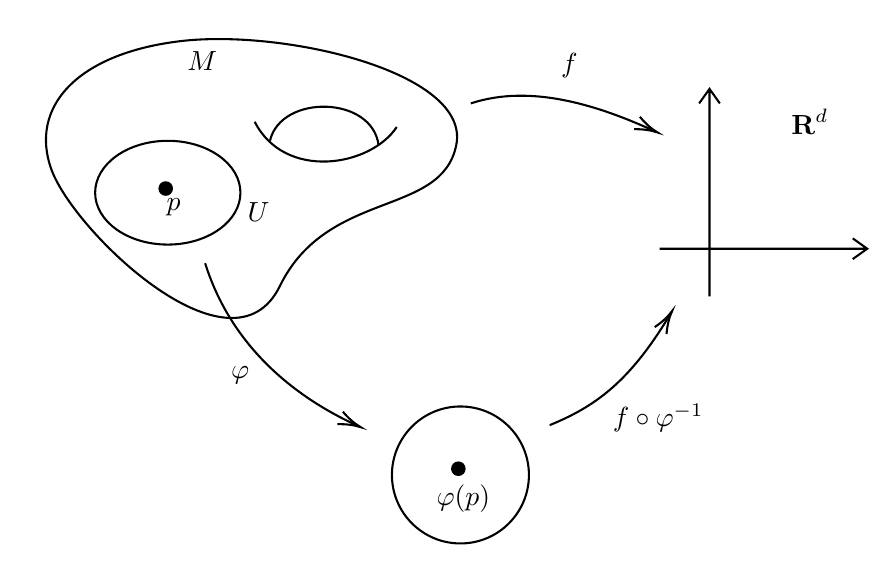
\begin{tikzpicture}[x=0.75pt,y=0.75pt,yscale=-1,xscale=1]
%uncomment if require: \path (0,436); %set diagram left start at 0, and has height of 436

%Shape: Polygon Curved [id:ds8701230940513227] 
\draw   (188,45) .. controls (238,39) and (328,60) .. (321,95) .. controls (314,130) and (259,116) .. (236,163) .. controls (213,210) and (137,137) .. (126,107) .. controls (115,77) and (138,51) .. (188,45) -- cycle ;
%Curve Lines [id:da00033147629047403093] 
\draw    (223.88,83.82) .. controls (238.3,112.28) and (279.62,105.58) .. (292.31,86.36) ;
%Curve Lines [id:da9461703131021257] 
\draw    (231.26,92.91) .. controls (236.56,70.44) and (280.47,71.1) .. (283.57,95.11) ;
%Shape: Ellipse [id:dp5760164398280032] 
\draw   (147,118) .. controls (147,104.19) and (162.67,93) .. (182,93) .. controls (201.33,93) and (217,104.19) .. (217,118) .. controls (217,131.81) and (201.33,143) .. (182,143) .. controls (162.67,143) and (147,131.81) .. (147,118) -- cycle ;
%Shape: Circle [id:dp35830362116000813] 
\draw  [fill={rgb, 255:red, 0; green, 0; blue, 0 }  ,fill opacity=1 ] (178,116) .. controls (178,114.34) and (179.34,113) .. (181,113) .. controls (182.66,113) and (184,114.34) .. (184,116) .. controls (184,117.66) and (182.66,119) .. (181,119) .. controls (179.34,119) and (178,117.66) .. (178,116) -- cycle ;

%Shape: Axis 2D [id:dp28763923911889777] 
\draw  (419,145) -- (519,145)(443,68) -- (443,168) (512,140) -- (519,145) -- (512,150) (438,75) -- (443,68) -- (448,75)  ;
%Shape: Circle [id:dp46748884211924646] 
\draw   (290,254) .. controls (290,235.77) and (304.77,221) .. (323,221) .. controls (341.23,221) and (356,235.77) .. (356,254) .. controls (356,272.23) and (341.23,287) .. (323,287) .. controls (304.77,287) and (290,272.23) .. (290,254) -- cycle ;
%Curve Lines [id:da19106736276909064] 
\draw    (200,152) .. controls (210.84,186.48) and (236.22,213.19) .. (273.3,230.23) ;
\draw [shift={(275,231)}, rotate = 204.1] [color={rgb, 255:red, 0; green, 0; blue, 0 }  ][line width=0.75]    (10.93,-3.29) .. controls (6.95,-1.4) and (3.31,-0.3) .. (0,0) .. controls (3.31,0.3) and (6.95,1.4) .. (10.93,3.29)   ;
%Shape: Circle [id:dp4052608591994611] 
\draw  [fill={rgb, 255:red, 0; green, 0; blue, 0 }  ,fill opacity=1 ] (319,251) .. controls (319,249.34) and (320.34,248) .. (322,248) .. controls (323.66,248) and (325,249.34) .. (325,251) .. controls (325,252.66) and (323.66,254) .. (322,254) .. controls (320.34,254) and (319,252.66) .. (319,251) -- cycle ;
%Curve Lines [id:da5944217136756031] 
\draw    (328,75) .. controls (357.4,65.2) and (390.64,76.53) .. (416.43,88.28) ;
\draw [shift={(418,89)}, rotate = 204.78] [color={rgb, 255:red, 0; green, 0; blue, 0 }  ][line width=0.75]    (10.93,-3.29) .. controls (6.95,-1.4) and (3.31,-0.3) .. (0,0) .. controls (3.31,0.3) and (6.95,1.4) .. (10.93,3.29)   ;
%Curve Lines [id:da8968041677982646] 
\draw    (366,230) .. controls (387.67,221.14) and (404.49,209.36) .. (424.1,176.52) ;
\draw [shift={(425,175)}, rotate = 120.47] [color={rgb, 255:red, 0; green, 0; blue, 0 }  ][line width=0.75]    (10.93,-3.29) .. controls (6.95,-1.4) and (3.31,-0.3) .. (0,0) .. controls (3.31,0.3) and (6.95,1.4) .. (10.93,3.29)   ;

% Text Node
\draw (180,119.4) node [anchor=north west][inner sep=0.75pt]    {$p$};
% Text Node
\draw (190,48.4) node [anchor=north west][inner sep=0.75pt]    {$M$};
% Text Node
\draw (219,121.4) node [anchor=north west][inner sep=0.75pt]    {$U$};
% Text Node
\draw (211,200.4) node [anchor=north west][inner sep=0.75pt]    {$\varphi $};
% Text Node
\draw (310,257.4) node [anchor=north west][inner sep=0.75pt]    {$\varphi ( p)$};
% Text Node
\draw (370,49.4) node [anchor=north west][inner sep=0.75pt]    {$f$};
% Text Node
\draw (395,218.4) node [anchor=north west][inner sep=0.75pt]    {$f\circ \varphi ^{-1}$};
% Text Node
\draw (481,76.4) node [anchor=north west][inner sep=0.75pt]    {${\displaystyle \mathbf{R}^{d}}$};


\end{tikzpicture}

    \caption{Smooth functions}
\end{figure}

\begin{remark}
    The smoothness of a function is independent of the choice of charts and is therefore well-defined (see Proposition \ref{lem:characterisation of smooth real-valued functions}).
\end{remark}

Smooth real-valued functions are important special case of smooth functions, we give the equivalent characterisation of smooth real-valued functions.

\begin{proposition}[Characterisation of smooth real-valued functions]\label{lem:characterisation of smooth real-valued functions}
    Let $M$ be a smooth manifold of dimension $n$, and let $f : M \to \mathbf{R}$ be a real-valued function. Then following are equivalent:
    \begin{enumerate}
        \item $f$ is $C^\infty$.
        \item The manifold $M$ has an atlas such that for every chart $(U, \varphi)$ in the atlas, one has $f \circ \varphi^{-1} : \varphi(U) \to \mathbf{R}$ is $C^\infty$.
        \item For every chart $(V, \psi)$ on $M$, $f \circ \psi^{-1} : \psi(V) \to \mathbf{R}$ is $C^\infty$.
    \end{enumerate}
\end{proposition}

\begin{proof}
    (i) $\Rightarrow$ (iii). Let $(V, \psi)$ be arbitrary chart on $M$ and $p \in V$. By definition, there exists a chart $(U, \varphi)$ containing $p \in U$ such that $f \circ \varphi^{-1}$ is $C^\infty$ at $\varphi(p) \in \varphi(U)$. We see that $f \circ \psi^{-1} = (f \circ \varphi^{-1}) \circ (\varphi \circ \psi^{-1})$ is $C^\infty$ at $\psi(p) \in \psi(U \cap V)$. Since $p \in V$ is arbitrary, $f \circ \psi^{-1}$ is $C^\infty$ on $\psi(V)$.

    (iii) $\Rightarrow$ (ii). This is trivial.

    (ii) $\Rightarrow$ (i). This is immediately comes from the definition.
\end{proof}

\subsection{Smooth maps between manifolds}

The definition of smooth functions generalizes easily to maps between manifolds.

\begin{definition}[Smooth map]
    Let $M$ and $N$ be smooth manifolds of dimension $n$ and $m$, respectively. Let $F : M \to N$ be a map. If $p \in M$, we say that $F$ is $C^\infty$ or \emph{smooth at $p$} if there exist charts $(U, \varphi)$ containing $p \in M$ and $(V, \psi)$ containing $F(p) \in N$ such that $F(U) \subset V$ and the composite $\psi \circ F \circ \varphi^{-1}$ is $C^\infty$ at $\varphi(p)$ from $\varphi(U)$ to $\psi(V)$. We say that $F$ is \emph{smooth} if it is smooth at every point of $M$.
\end{definition}

\begin{figure}[h]
    \centering
    


\tikzset{every picture/.style={line width=0.75pt}} %set default line width to 0.75pt        

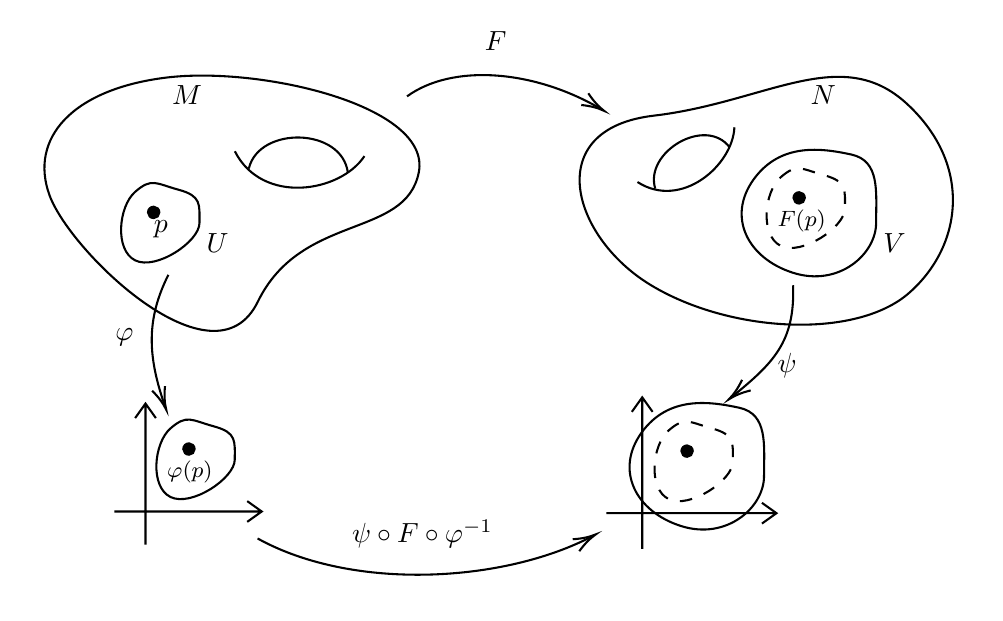
\begin{tikzpicture}[x=0.75pt,y=0.75pt,yscale=-1,xscale=1]
%uncomment if require: \path (0,308); %set diagram left start at 0, and has height of 308

%Shape: Polygon Curved [id:ds6525401307539842] 
\draw   (172.32,39.91) .. controls (217.93,34.42) and (300.03,53.64) .. (293.65,85.68) .. controls (287.26,117.72) and (237.09,104.91) .. (216.11,147.93) .. controls (195.13,190.95) and (125.8,124.13) .. (115.76,96.67) .. controls (105.73,69.21) and (126.71,45.41) .. (172.32,39.91) -- cycle ;
%Curve Lines [id:da13910221661848143] 
\draw    (205.05,75.45) .. controls (218.2,101.5) and (255.9,95.36) .. (267.47,77.78) ;
%Curve Lines [id:da7264884996321357] 
\draw    (211.78,83.77) .. controls (216.62,63.2) and (256.67,63.81) .. (259.5,85.79) ;
%Shape: Ellipse [id:dp09144271455218123] 
\draw  [fill={rgb, 255:red, 0; green, 0; blue, 0 }  ,fill opacity=1 ] (163.2,104.91) .. controls (163.2,103.39) and (164.42,102.16) .. (165.94,102.16) .. controls (167.45,102.16) and (168.67,103.39) .. (168.67,104.91) .. controls (168.67,106.42) and (167.45,107.65) .. (165.94,107.65) .. controls (164.42,107.65) and (163.2,106.42) .. (163.2,104.91) -- cycle ;

%Curve Lines [id:da40516895320740165] 
\draw    (399.04,90.27) .. controls (420.05,103.85) and (444.95,82.27) .. (445.73,63.89) ;
%Shape: Polygon Curved [id:ds6664506251612305] 
\draw   (406.83,58.3) .. controls (461.29,51.9) and (497.08,23.13) .. (528.98,52.7) .. controls (560.89,82.27) and (555.44,121.43) .. (529.76,143.81) .. controls (504.09,166.19) and (443.39,162.99) .. (405.27,139.81) .. controls (367.14,116.64) and (352.36,64.69) .. (406.83,58.3) -- cycle ;
%Curve Lines [id:da7681269690042121] 
\draw    (407.6,93.46) .. controls (402.16,75.88) and (431.72,58.3) .. (443.39,73.48) ;
%Shape: Polygon Curved [id:ds13343779797680644] 
\draw   (157,95) .. controls (165,88) and (167,91) .. (178,94) .. controls (189,97) and (188,101) .. (188,110) .. controls (188,119) and (167,133) .. (157,128) .. controls (147,123) and (149,102) .. (157,95) -- cycle ;
%Shape: Polygon Curved [id:ds6611856882220029] 
\draw   (455,89) .. controls (468,71) and (488,74) .. (502,77) .. controls (516,80) and (514,95) .. (514,110) .. controls (514,125) and (496,141) .. (474,134) .. controls (452,127) and (442,107) .. (455,89) -- cycle ;
%Curve Lines [id:da20913952032416394] 
\draw    (288,49) .. controls (309.67,33.24) and (348.8,35.91) .. (381.51,55.11) ;
\draw [shift={(383,56)}, rotate = 211.22] [color={rgb, 255:red, 0; green, 0; blue, 0 }  ][line width=0.75]    (10.93,-3.29) .. controls (6.95,-1.4) and (3.31,-0.3) .. (0,0) .. controls (3.31,0.3) and (6.95,1.4) .. (10.93,3.29)   ;
%Shape: Ellipse [id:dp28625789196692764] 
\draw  [fill={rgb, 255:red, 0; green, 0; blue, 0 }  ,fill opacity=1 ] (180.2,218.91) .. controls (180.2,217.39) and (181.42,216.16) .. (182.94,216.16) .. controls (184.45,216.16) and (185.67,217.39) .. (185.67,218.91) .. controls (185.67,220.42) and (184.45,221.65) .. (182.94,221.65) .. controls (181.42,221.65) and (180.2,220.42) .. (180.2,218.91) -- cycle ;
%Shape: Polygon Curved [id:ds6638368612589451] 
\draw   (174,209) .. controls (182,202) and (184,205) .. (195,208) .. controls (206,211) and (205,215) .. (205,224) .. controls (205,233) and (184,247) .. (174,242) .. controls (164,237) and (166,216) .. (174,209) -- cycle ;
%Curve Lines [id:da41107146503736036] 
\draw    (173,135) .. controls (162.27,156.45) and (162.96,174.1) .. (171.34,198.14) ;
\draw [shift={(172,200)}, rotate = 250.2] [color={rgb, 255:red, 0; green, 0; blue, 0 }  ][line width=0.75]    (10.93,-3.29) .. controls (6.95,-1.4) and (3.31,-0.3) .. (0,0) .. controls (3.31,0.3) and (6.95,1.4) .. (10.93,3.29)   ;
%Shape: Ellipse [id:dp45763550840932554] 
\draw  [fill={rgb, 255:red, 0; green, 0; blue, 0 }  ,fill opacity=1 ] (474.2,97.91) .. controls (474.2,96.39) and (475.42,95.16) .. (476.94,95.16) .. controls (478.45,95.16) and (479.67,96.39) .. (479.67,97.91) .. controls (479.67,99.42) and (478.45,100.65) .. (476.94,100.65) .. controls (475.42,100.65) and (474.2,99.42) .. (474.2,97.91) -- cycle ;
%Shape: Polygon Curved [id:ds9301475980831604] 
\draw  [dash pattern={on 4.5pt off 4.5pt}] (468,88) .. controls (476,81) and (478,84) .. (489,87) .. controls (500,90) and (499,94) .. (499,103) .. controls (499,112) and (478,126) .. (468,121) .. controls (458,116) and (460,95) .. (468,88) -- cycle ;
%Curve Lines [id:da1605123699723061] 
\draw    (474,140) .. controls (474.98,167.44) and (464.44,177.59) .. (444.25,193.99) ;
\draw [shift={(443,195)}, rotate = 321.01] [color={rgb, 255:red, 0; green, 0; blue, 0 }  ][line width=0.75]    (10.93,-3.29) .. controls (6.95,-1.4) and (3.31,-0.3) .. (0,0) .. controls (3.31,0.3) and (6.95,1.4) .. (10.93,3.29)   ;
%Curve Lines [id:da5075807557158749] 
\draw    (216,262) .. controls (262.53,287.74) and (335.52,283.1) .. (377.73,260.68) ;
\draw [shift={(379,260)}, rotate = 151.29] [color={rgb, 255:red, 0; green, 0; blue, 0 }  ][line width=0.75]    (10.93,-3.29) .. controls (6.95,-1.4) and (3.31,-0.3) .. (0,0) .. controls (3.31,0.3) and (6.95,1.4) .. (10.93,3.29)   ;
%Shape: Axis 2D [id:dp1641739751745317] 
\draw  (147,249) -- (218,249)(162,197) -- (162,265) (211,244) -- (218,249) -- (211,254) (157,204) -- (162,197) -- (167,204)  ;
%Shape: Axis 2D [id:dp7431220916836756] 
\draw  (384,249.82) -- (466,249.82)(401.32,194) -- (401.32,267) (459,244.82) -- (466,249.82) -- (459,254.82) (396.32,201) -- (401.32,194) -- (406.32,201)  ;
%Shape: Polygon Curved [id:ds06622774826865241] 
\draw   (401,211) .. controls (414,193) and (434,196) .. (448,199) .. controls (462,202) and (460,217) .. (460,232) .. controls (460,247) and (442,263) .. (420,256) .. controls (398,249) and (388,229) .. (401,211) -- cycle ;
%Shape: Ellipse [id:dp6760122392287706] 
\draw  [fill={rgb, 255:red, 0; green, 0; blue, 0 }  ,fill opacity=1 ] (420.2,219.91) .. controls (420.2,218.39) and (421.42,217.16) .. (422.94,217.16) .. controls (424.45,217.16) and (425.67,218.39) .. (425.67,219.91) .. controls (425.67,221.42) and (424.45,222.65) .. (422.94,222.65) .. controls (421.42,222.65) and (420.2,221.42) .. (420.2,219.91) -- cycle ;
%Shape: Polygon Curved [id:ds3192888406480947] 
\draw  [dash pattern={on 4.5pt off 4.5pt}] (414,210) .. controls (422,203) and (424,206) .. (435,209) .. controls (446,212) and (445,216) .. (445,225) .. controls (445,234) and (424,248) .. (414,243) .. controls (404,238) and (406,217) .. (414,210) -- cycle ;

% Text Node
\draw (173.36,42.38) node [anchor=north west][inner sep=0.75pt]    {$M$};
% Text Node
\draw (190,113.4) node [anchor=north west][inner sep=0.75pt]    {$U$};
% Text Node
\draw (164.5,107.38) node [anchor=north west][inner sep=0.75pt]    {$p$};
% Text Node
\draw (324,16.4) node [anchor=north west][inner sep=0.75pt]    {$\mathnormal{F}$};
% Text Node
\draw (170.94,223.05) node [anchor=north west][inner sep=0.75pt]  [font=\footnotesize]  {$\varphi ( p)$};
% Text Node
\draw (146,159.4) node [anchor=north west][inner sep=0.75pt]    {$\varphi $};
% Text Node
\draw (481,42.4) node [anchor=north west][inner sep=0.75pt]    {$\mathnormal{N}$};
% Text Node
\draw (465,102.4) node [anchor=north west][inner sep=0.75pt]  [font=\footnotesize]  {$F( p)$};
% Text Node
\draw (516,113.4) node [anchor=north west][inner sep=0.75pt]    {$V$};
% Text Node
\draw (465,171.4) node [anchor=north west][inner sep=0.75pt]    {$\psi $};
% Text Node
\draw (260,251.4) node [anchor=north west][inner sep=0.75pt]    {$\psi \circ F\circ \varphi ^{-1}$};


\end{tikzpicture}

    \caption{Smooth maps}
\end{figure}

\begin{comment}
We show now that smoothness implies continuity, and that the smoothness of a map is independent of the choice of charts.

\begin{lemma}\label{lem:smooth map is continuous}
    Let $M, N$ be smooth manifolds, and let $F : M \to N$ be a smooth map.
    \begin{enumerate}
        \item If $(U, \varphi)$ is arbitrary chart containing $p \in M$ and $(V, \psi)$ is arbitrary chart containing $F(p) \in N$, then $\psi\circ F \circ \varphi^{-1}$ is $C^\infty$ on $M$.
    \end{enumerate}
\end{lemma}

\begin{proof}
    (i) Let $p \in M$ be arbitrary. Suppose that $F$ is smooth at $p$. By definition, there are charts $(U, \varphi)$ containing $p \in M$ and $(V, \psi)$ containing $F(p) \in N$ such that $F(U) \subset V$ and the composite $\psi \circ F \circ \varphi^{-1}$ is $C^\infty$ at $\varphi(p)$ from $\varphi(U)$ to $\psi(V)$, hence $F$ is continuous on $\varphi(U)$. Since $\varphi : U \to \varphi(U)$ and $\psi : V \to \psi(V)$ are homeomorphisms, then the composite of continuous maps $F = \psi^{-1} \circ (\psi \circ F \circ \varphi^{-1}) \circ \varphi$ from $U$ to $V$ is also continuous. Since $p$ is arbitrary, $F$ is continuous.
\end{proof}
\end{comment}

\begin{proposition}[Characterisation of smooth maps]\label{lem:characterisation of smooth maps}
    Let $M$ and $N$ be smooth manifolds, and let $F : M \to N$ be a map. Then following are equivalent:
    \begin{enumerate}
        \item $F$ is $C^\infty$.
        \item For every $p \in M$, there exist charts $(U, \varphi)$ containing $p$ and $(V, \psi)$ containing $F(p)$ such that $U \cap F^{-1}(V)$ is open in $M$ and the composite map $\psi \circ F \circ \varphi^{-1}$ is $C^\infty$ from $\varphi(U \cap F^{-1}(V))$ to $\psi(V)$.
        \item $F$ is continuous and there exist atlases $\mathfrak{A}$ for $M$ and $\mathfrak{B}$ for $N$ such that for every chart $(U_\alpha, \varphi_\alpha) \in \mathfrak{A}$ and $(V_\beta, \psi_\beta) \in \mathfrak{B}$, $\psi_\beta \circ F \circ \varphi_\alpha^{-1}$ is $C^\infty$ from $\varphi_\alpha(U_\alpha \cap F^{-1}(V_\beta))$ to $\psi_\beta(V_\beta)$.
        %\item For every chart $(U, \varphi)$ on $M$ and $(V, \psi)$ on $N$, the map $\psi \circ F \circ \varphi^{-1}$ is $C^\infty$ from $\varphi(U \cap F^{-1}(V))$ to $\psi(V)$.
    \end{enumerate}
\end{proposition}

\begin{proof}
    (i) $\Rightarrow$ (ii). Suppose $F$ is $C^\infty$. Let $p \in M$ be arbitrary, then there exist charts $(U, \varphi)$ containing $p$ and $(V, \psi)$ containing $F(p)$ such that $F(U) \subset V$ and the composite $\psi \circ F \circ \varphi^{-1}$ is $C^\infty$ at $\varphi(p)$ from $\varphi(U)$ to $\psi(V)$. Since for every $x \in M$ and every chart $(V, \psi)$ such that $F(p) \in V$, we have $x \in U$ and $F(U) \subset V$, $F$ is continuous. This implies that $F^{-1}(V)$ is open in $M$ for $V$ is open in $N$, hence $U \cap F^{-1}(V)$ is open in $M$. Obviously, $p \in U \cap F^{-1}(V)$ for that $F(p) \in V$. Since $\varphi(U \cap F^{-1}(V)) \subset \varphi(U)$, $\psi \circ F \circ \varphi^{-1}$ is also $C^\infty$ at $\varphi(p)$ from $\varphi(U \cap F^{-1}(V))$ to $\psi(V)$. Because $p \in M$ is arbitrary, the claim follows.

    (ii) $\Rightarrow$ (iii).  We only need to show that $F$ is continuous, the remaining part is trivial. Since for every $p \in M$ there is a chart $(V, \psi)$ such that $F(p) \in V$. Then for $p \in U \cap F^{-1}(V)$, we have $F(U \cap F^{-1}(V)) \subset F(U) \cap F(F^{-1}(V)) \subset F(U) \cap V \subset V$. Thus $F$ is continuous. 

    (iii) $\Rightarrow$ (i). Suppose (iii) and let $U = U_\alpha \cap F^{-1}(V_\beta) \subset U_\alpha$. Then we obtain $(U, \varphi_\alpha|_U)$ such that (iii) holds which is easy to prove. From the continuity of $F$, we have $F(U) \subset V_\beta$ is open. This close the proof.
    \begin{comment}
    (ii) $\Rightarrow$ (iv). Let $(\widetilde{U}, \widetilde{\varphi})$ and $(\widetilde{V}, \widetilde{\psi})$ be any charts on $M$ and $N$, respectively, such that $\widetilde{U} \cap F^{-1}(\widetilde{V}) \neq \emptyset$. If $p \in \widetilde{U} \cap F^{-1}(\widetilde{V})$. by assumption, there are charts $(U, \varphi)$ containing $p$ and $(V, \psi)$ containing $F(p)$ such that  $\psi \circ F \circ \varphi^{-1}$ is $C^\infty$ from $\varphi(U \cap F^{-1}(V))$ to $\psi(V)$. By the $C^\infty$-compatibility of charts in a differentiable structure, $\varphi \circ \widetilde{\varphi}^{-1} : \widetilde{\varphi}(U \cap \widetilde{U}) \to \varphi(U \cap \widetilde{U})$ and $\widetilde{\psi} \circ \psi^{-1} : \psi(V \cap \widetilde{V}) \to \widetilde{\psi}(V \cap \widetilde{V})$ are $C^\infty$. Thus,
    \begin{align*}
        \widetilde{\psi} \circ F \circ \widetilde{\varphi}^{-1}
        = (\widetilde{\psi} \circ \psi^{-1}) \circ
        (\psi \circ F \circ \varphi^{-1}) \circ
        (\varphi \circ \widetilde{\varphi}^{-1})
    \end{align*}
    is $C^\infty$ at $\widetilde{\varphi}(p)$. Since $p \in \widetilde{U} \cap F^{-1}(\widetilde{V})$ is arbitrary, so does $\widetilde{\varphi}(p) \in \widetilde{\varphi}(\widetilde{U} \cap F^{-1}(\widetilde{V}))$, we have $\widetilde{\psi} \circ F \circ \widetilde{\varphi}^{-1}$ is $C^\infty$ from $\widetilde{\varphi}(\widetilde{U} \cap F^{-1}(\widetilde{V}))$ to $\widetilde{\psi}(\widetilde{V})$.
    \end{comment}
\end{proof}

Above proposition shows that the smoothness implies continuity. As a corollary of above conclusion, we see that the smoothness of maps is independent of the choice of charts.

\begin{corollary}\label{lem:smoothness is independent of chars}
    Let $M, N$ be smooth manifolds, and let $F : M \to N$ be a smooth map. If $(U, \varphi)$ is arbitrary chart containing $p \in M$ and $(V, \psi)$ is arbitrary chart containing $F(p) \in N$, then $\psi\circ F \circ \varphi^{-1}$ is $C^\infty$ on $M$.
\end{corollary}

\begin{proof}
    Let $(\widetilde{U}, \widetilde{\varphi})$ and $(\widetilde{V}, \widetilde{\psi})$ be arbitrary charts for $M$. Suppose that $\widetilde{U} \cap F^{-1}(\widetilde{V}) \neq \emptyset$. Since $F$ is smooth, for $p \in \widetilde{U} \cap F^{-1}(\widetilde{V}) \subset M$, there exist charts $(U, \varphi)$ containing $p$ and $(V, \psi)$ containing $F(p)$ such that $\psi \circ F \circ \varphi^{-1}$ is $C^\infty$ at $\varphi(p)$ on $\varphi(U \cap F^{-1}(V))$. By the $C^\infty$-compatibility of charts in a differentiable structure, we have $\widetilde{\psi} \circ F \circ \widetilde{\varphi}^{-1} = (\widetilde{\psi} \circ \psi^{-1}) \circ (\psi \circ F \circ \varphi^{-1}) \circ (\varphi \circ \widetilde{\varphi}^{-1})$ is $C^\infty$ at $\widetilde{\varphi}(p)$ on $\widetilde{\varphi}(\widetilde{U} \cap F^{-1}(\widetilde{V}))$. Since $(\widetilde{U}, \widetilde{\varphi})$ and $(\widetilde{V}, \widetilde{\psi})$ are arbitrary, the claim follows.
\end{proof}

\subsection{Constructing smooth maps}

How does one go about constructing smooth maps from one smooth manifold to another? Following theorem gives a number of rules for constructing smooth maps.

\begin{theorem}[Construction of smooth maps]\label{lem:construction of smooth maps}
    Let $M, N$ and $P$ be smooth manifolds.
    \begin{enumerate}
        \item (Constant map) Every constant map $f : M \to N$ is smooth.
        \item (Identity map) The identity map $\id_M$ is smooth.
        \item (Composites) If $F : M \to N$ and $G : N \to P$ are smooth, then $G \circ F : M \to P$ is smooth.
        %\item (Restriction) $F : M \to N$ is smooth if and only if very point $p \in M$ has a neighborhood $U$ such that $F|_U : U \to N$ is smooth.
    \end{enumerate}
\end{theorem}

\begin{proof}
    (i) Define $f : M \to N$ as $f(p) = c$. Let $p \in M$ be arbitrary, there exist charts $(U, \varphi)$ containing $p \in M$ and $(V, \psi)$ containing $c$. We see that $U \cap f^{-1}(V) = U \cap M = U$ is open in $M$ and $\psi \circ f \circ\varphi^{-1}$ is $C^\infty$ from $\varphi(U)$ to $\psi(V)$. Thus, $f$ is $C^\infty$.

    (ii) Let $p \in M$ be arbitrary, there exist $(U, \varphi)$ containing $p$. Then $U \cap \id_M^{-1}(U) = U$ is open in $M$ and $\varphi \circ \id_M \circ \varphi^{-1}$ is $C^\infty$ from $\varphi(U)$ to $\varphi(U)$. Thus, $\id_M$ is $C^\infty$.

    (iii) By definition, there exist charts $(V, \varrho)$ containing $F(p)$ and $(W, \psi)$ containing $G(F(p))$ such that $G(V) \subset W$ and $\psi \circ G \circ \varrho^{-1}$ is $C^\infty$ from $\varrho(V)$ to $\psi(W)$. Since $F$ is continuous and $F^{-1}(V)$ is a neighborhood of $p \in M$, so there is a chart $(U, \varphi)$ for $M$ such that $p \in U \subset F^{-1}(V)$. By Corollary \ref{lem:smoothness is independent of chars}, $\psi \circ F \circ \varphi^{-1}$ is $C^\infty$ from $\varphi(U)$ to $\psi(V)$. Then we have $(G \circ F)(U) \subset G(U) \subset W$, and $\varrho \circ (G \circ F) \circ \varphi^{-1} = (\varrho \circ G \circ \psi^{-1}) \circ (\psi \circ F \circ \varphi^{-1})$ is $C^\infty$ from $\varphi(U)$ to $\varrho(W)$.
\end{proof}

\section{Diffeomorphisms}

\begin{definition}[Diffeomorphism]
    Let $M$ and $N$ be smooth manifolds. A \emph{diffeomorphism from $M$ to $N$} is a bijective smooth map $F : M \to N$ whose inverse $F^{-1}$ is also smooth. We say that $M$ and $N$ are \emph{diffeomorphic} if there exists a diffeomorphism between them.
\end{definition}

Following proposition gives the relation between diffeomorphism and chart.

\begin{proposition}\label{lem:chart map is diffeomorphism}
    Let $M$ be a smooth manifold. If $(U, \varphi)$ is a chart on $M$, then $\varphi : U \to \varphi(U)$ is a diffeomorphism. Conversely, if $\varphi : U \to \varphi(U)$ is a diffeomorphism on the open subset $U \subset M$, then $(U, \varphi)$ is a chart in the differentiable structure of $M$.
\end{proposition}

\begin{proof}
    Suppose that $(U, \varphi)$ is a chart on $M$, then by definition, $\varphi : U \to \varphi(U)$ is a homeomorphism. We need to show that $\varphi$ and $\varphi^{-1}$ is $C^\infty$. Consider the atlases $\{(U, \varphi)\}$ and $\{(\varphi(U), \id_{\varphi(U)})\}$ which contains single chart. Since $\varphi$ and $\varphi^{-1}$ are continuous, and $\id_{\varphi(U)} \circ \varphi \circ \varphi^{-1}$ and $\varphi \circ \varphi^{-1} \circ \id_{\varphi(U)}$ are identity maps on $\varphi(U)$ and $U$, respectively. Thus, by Theorem \ref{lem:construction of smooth maps}(ii) and Proposition \ref{lem:characterisation of smooth maps}(iii), $\varphi$ and $\varphi^{-1}$ are $C^\infty$.

    Conversely, suppose that $U \subset M$ is open and $\varphi : U \to \varphi(U)$ is diffeomorphism. Then by definition, $\varphi$ and $\varphi^{-1}$ are $C^\infty$. For any chart $(V, \psi)$ in maximal atlas $\mathfrak{A}$ of $M$, we have $\psi$ and $\psi^{-1}$ are $C^\infty$ from above conclusion. Then by Theorem \ref{lem:construction of smooth maps}(iii), $\varphi \circ \psi^{-1} : \psi(U \cap V) \to \varphi(U \cap V)$ and $\psi \circ \varphi^{-1} : \varphi(U \cap V) \to \psi(U \cap V)$ are $C^\infty$. This means that $(U, \varphi)$ is compatible with $(V, \psi)$. Since $(V, \psi)$ is arbitrary, $(U, \varphi) \in \mathfrak{A}$, as desired.
\end{proof}
